\begin{figure}[htbp]
\centering
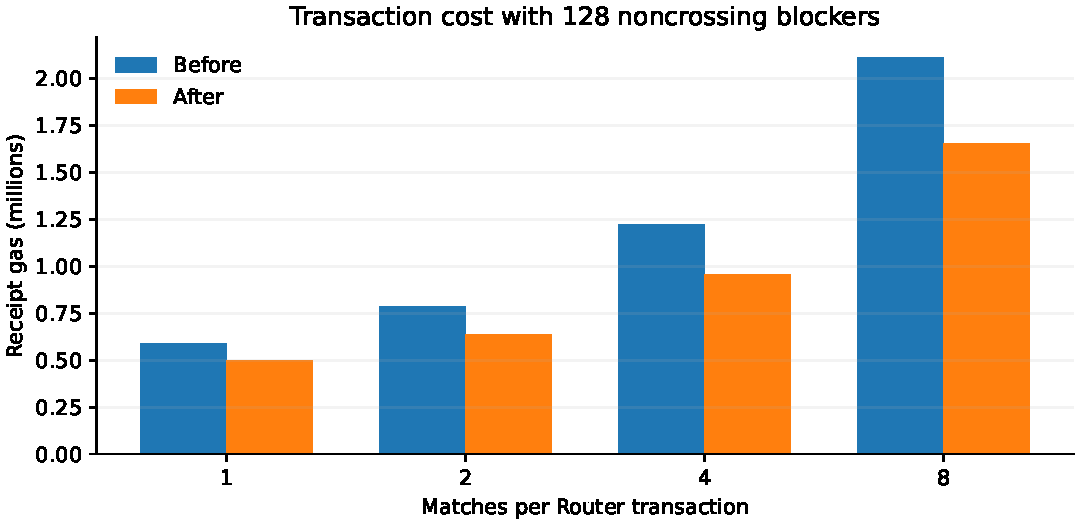
\includegraphics[width=0.85\textwidth]{figures/matching-receipts.pdf}
\caption{Actual Router transaction receipts, including intrinsic gas and applied storage refunds.}
\end{figure}
\begin{center}
\begin{tabular}{r r r r}
\hline
Matches & Before & After & Reduction \\
\hline
1 & 586,379 & 500,583 & 14.6\% \\
2 & 786,552 & 636,940 & 19.0\% \\
4 & 1,220,974 & 955,580 & 21.7\% \\
8 & 2,110,075 & 1,652,381 & 21.7\% \\
\hline
\end{tabular}
\end{center}
These are separate \texttt{Router.matchBook} transactions on a local Anvil, each starting from
an imported Foundry fixture with 128 blockers and 32 crossing pairs, standard ERC-20 tokens,
and no LP positions. All emitted events agree before and after optimization. Receipt gas
includes intrinsic gas and applied refunds; it must not be compared directly with the gross
unlock measurements above. One match is cheaper in total than eight, while eight amortizes
entry costs across more matches. Different owners, token implementations, LP state, partial
fills, and tree shapes can change these costs. The measurements do not establish a global
minimum or a worst-case gas limit.

Both versions use Solidity 0.8.26 with 43,690 optimizer runs.
